% ------- Create Preamble ------------
\documentclass [12pt]{article} 
\usepackage[a4paper]{geometry} 
\usepackage{amsmath, amsthm, amssymb, amsfonts}
 \usepackage{graphicx,epsfig}
\usepackage{booktabs} 
\usepackage{pslatex} 
\usepackage{caption} 
\usepackage{setspace} 
\usepackage[pagebackref]{hyperref} 
\usepackage[noabbrev, nameinlink]{cleveref}
\usepackage{multicol, multirow}
\usepackage{graphicx,epsfig}
\usepackage{booktabs}
\usepackage{pslatex}
\usepackage{caption}
\usepackage[capposition=top]{floatrow}
\usepackage{textgreek}
\usepackage{pdfpages}
\usepackage{apacite}
\usepackage{floatrow}
\usepackage{mdframed}
\usepackage{natbib} % For references
\bibpunct{(}{)}{;}{a}{}{,} % Reference punctuation
\def\citeapos#1{\citeauthor{#1}'s (\citeyear{#1})}
\newtheorem{hypothesis}{Hypothesis}
\newtheorem{nullhypothesis}{Null Hypothesis}
\usepackage{xcolor}
\hypersetup{
    colorlinks,
    linkcolor={blue!50!blue},
    citecolor={blue!50!blue},
    urlcolor={blue!50!blue}
}

\usepackage{tikz}
\usetikzlibrary{shapes.geometric, arrows}
\tikzstyle{startstop} = [rectangle, rounded corners, minimum width=3cm, minimum height=1cm,text centered, draw=black, fill=white]
\tikzstyle{io} = [rectangle, rounded corners, minimum width=3cm, minimum height=1cm,text centered, draw=black, fill=white]
\tikzstyle{io2} = [rectangle, rounded corners, minimum width=3cm, minimum height=1cm,text centered, draw=black, fill=white]
\tikzstyle{arrow} = [thick,->,>=stealth]

\usepackage{booktabs}
\usepackage{siunitx}
\newcolumntype{d}{S[input-symbols = ()]}

%---Set up author and title page
\singlespace
\title{Snap judgements, emotion, and learning about politics}
\author{Damon C.\ Roberts\footnote{Ph.D Candidate,
Department of Political Science, University of Colorado Boulder, UCB 333, Boulder, CO 80309-0333. Damon.Roberts-1@colorado.edu.}}

%set up document
\date{\today}
\begin{document}
\maketitle


\newpage
\doublespace
\newpage
\section*{Introduction}

\begin{quote}
    ``All perceiving is also thinking, all reasoning is also intuition, all observation is also invention'' - Rudolf Arnheim
\end{quote}

Imagine we are at the airport and we see a bright red had with white lettering on it. You have well-trodden neurological paths of what the color red looks like, what a hat looks like, and what a hat with white lettering looks like. You are accessing associative memory to not just imagine what each of these pieces of information look like in isolation, but you likely have seen these features in combination before. So rather than just seeing these details, you likely are filling in other gaps too by relying on memory.

Memories are easier to retrieve if they are recent, contiguous (associated with other pieces of information), similar to the information that made them ``hot'', are reinforced, and have primacy over other pieces of information \citep{kahana_et-al_2022_ohhum}. What this means is that the visual information of a red hat with white lettering likely spark memories by which you've recently seen a hat with similar features.

Given that you are reading a prospectus for a political scientist's dissertation, the contextual state you are in may have prompted you to imagine this hat as being related to politics in some way as opposed to belonging to an Arsenal F.C. fan. Because of its similarity with the ``Make America Great Again'' hat which have become a characteristic symbol of the Republican party in the post-Trump era, this information may have sparked your brain to access such a memory of what a MAGA hat looks like. 

An important contextual feature of memory is the affective state by which you associate with it. Memories are enhanced when they are ``tagged'' with affective information \citep{kensinger_fields_2022_ohhum}. When converting perceived visual information to a memory, emotion moderates the encoding, consolidation, and retrieval stages \citep{kensinger_fields_2022_ohhum}. This means that when you process the visual information of a red hat with white lettering, and you access memories which suggest that it should be a hat representing support for Donald Trump, you retrieve memories that are associated with and trigger a strong autonomic physiological reaction. In response, your brain will contact your limbic system to appraise that particular physiological response and to label it based on memories that associate physiological responses with an affective state \citep{valentino_et-al_2011_jop}.

The link between affective state and physiological response encourages a corresponding behavioral response \citep{valentino_et-al_2011_jop}. If you connect that the hat belongs to a Trump supporter, you may have a physiological reaction of feeling queasy, an increase in heart rate, and your hands may feel clammy. As these reactions are characteristic of disgust, you may feel an urge to avoid such a person. 

It may be the case that when you board your plane, this person may be in the seat next to you. You realize that despite this urge for you to avoid them, you nonetheless will likely have to exchange a few niceties at the very least. So long as you avoid talking about politics, you might be able to escape without feeling any worse by managing to avoid getting in a disagreement with someone \citep{mutz_2006, carlson_settle_2022_cup}. Despite your best intentions, they begin talking to you, and they jump right into talking about baseball, your favorite sport! The conversation ends up being an engaging one. Your initial intentions of avoiding them are changing. Your initial negative evaluation of that person dissipates and may even turn into a positive one. This is likely short-lived however \citep{santoro_broockman_2022_sa}. This is because the memories associating a negative affective state with a Trump supporter are stronger than a brief conversation with one about a common interest, so that memory is crowded out and eventually purged as time goes on \citep{kahana_et-al_2022_ohhum}.


The snap-judgement model expands upon the popular memory and online dual-processing models in political psychology. The snap-judgement model asserts that it is visual information such as color and shapes that individuals rely on first to process politically-relevant information. It is not limited to examining text-based information as is common in many political science experiments that rely on text-based vignettes. From an evolutionary perspective, humans are attuned and adept at detecting and finding meaning from images. From a neurological perspective, processing visual information is much faster as it occurs simultaneously in different parts of the brain as opposed to text which takes a more linear path \citep{vogel_et-al_1986_wp}. Some estimates suggest that visual information can take as little as 13 milliseconds to be perceived \citep{potter_et-al_2014_app}. Visual information is not \textit{just} processed quicker, but it tends to have potency.

Visual information contains powerful meaning via affect. Visual information such as color contain important affective associations \citep{cimbalo_et-al_1978_jgp}. Memory associated with affect pass through the limbic system which mean that they are often easily and quickly encoded, easier to consolidate by placing it in an associative memory network, and will be easier to retrieve later \citep{kensinger_fields_2022_ohhum}. Simple visual information, like color, are referential in this way \citep{elliot_maier_2012_aesp}. Republicans report that they prefer ``Republican red'' more than they do than ``Democratic blue''; it engenders an affective response that is rooted in identity.

Political symbology is common in politics and performs a significant role in shaping attitudes and behaviors. This symbology is often consumed in a variety of complex contexts. Strong partisans use yard signs as an expressive act which often succeed at generating valanced reactions from their neighbors \citep{makse_et-al_2019_oup}. Even in seemingly non-political ways, observing stereotyped cultural differences between Republicans and Democrats act as relatively accurate visual cues - such as the modal car in the driveway - of any given neighborhood to assume the partisan composition of those who live there \citep{hetherington_weiler_2018_hmh}.

Connecting the literature on affective memory to existing work in political science on visual information yields the snap-judgement model. Going back to the example of the ``MAGA hat" exercise, the ``laws'' of recency, contiguity, and repetition \citep{kahana_et-al_2022_ohhum} would suggest that a simple prompt of red hat with white lettering would evoke a particular image. ``MAGA hats'' are a new but very prominent symbol representing the political views of the Trump-era Republican party. This means that it is easier to recall a ``MAGA hat'' than a hat with similar characteristics you may have seen years ago. With repetition, the connection is strengthened so that now, you are more likely to assume that I am describing a MAGA hat. As this visual information is encoded, so is the context. This means that when retrieving visual memories of a red hat with white lettering, contiguous neurological networks consolidating other visual information are retrieved as well. This means with memories of red hats with white lettering, you are more likely to recall other contextual information, e.g., the wearer of the hat and the meaning of the political views of those owning such a hat. As individuals have affective reactions to either congruent or incongruent political views \citep{iyengar_westwood_2015, druckman_levendusky_2019}, these memories should also be higher priority in that encoding, consolidation, and retrieval should be easier than other neutral visual information \citep{kensinger_fields_2022_ohhum}. 

The snap-judgement model expands upon extant theories of political information processing. The two leading theories of political information processing are \citeauthor{zaller_1992}'s \citeyearpar{zaller_1992} memory-based model and \citeauthor{lodge_taber_2013_cup}'s \citeyearpar{lodge_taber_2013_cup} online model. Both models present John Q. Public as a bayesian updater. The memory-based model presents JQP as one with a very weak prior that is amendable to change with new political information. The memory-based model presents JQP as one who evaluates this information rationally; that is, consciously. The online model suggests that JQP heavily relies on their priors and will largely ignore new information that is not congruent with the prior. It does this by arguing that new information sparks an automatic affective pre-conscious reaction that has downstream effects for the rest of the process. These models are agnostic to the type of information their models apply to.

The snap-judgment model is also one that is largely rooted in the role of pre-conscious information processing. It agrees with the online model in that stimuli engender an automatic affective response which direct the neurological path for pre-conscious processing. It theorizes, however, about the way in which these snap-judgments are mediated by other information such as context and interactions with the stimulant. The implication of this is that rather than concluding with motivated reasoning and continued polarization of political attitudes, it suggests conditions under which learning and persuasion occur.

The snap-judgement model highlights a subsystem of information processing. Once an individual forms a snap-judgement, their priors will take over and the affective reaction will activate a particular behavioral response. However, when incorrect appraisals or an intervening factor that attenuates the cognitive disengagement occurs, it may act as a valuable learning lesson that might have an opposite effect. As affective tagging of information can occur later \citep{kensinger_fields_2022_ohhum}, a positive experience, despite a negative snap-judgement, may weaken the association of a visual object with a negative affective response. Some evidence suggests that such a mechanism is plausible \citep{santoro_broockman_2022_sa}. As evidence suggests these depolarizing effects tend to be short term \citep{santoro_broockman_2022_sa}, the snap-judgement model suggests that this is due to the case that such interactions are not often reinforced. Without reinforcement, those memories are purged and the dampening effects are removed \citep[see][]{kahana_et-al_2022_ohhum}. It may be the case, however, that these are not all too common as individuals tend to avoid engaging with an object representing ideologically incongruent positions \citep[see][]{mutz_2006, klar_krupnikov_2016}.

\Cref{fig:snap-judgement_model} presents a summary of the snap-judgement model. This dissertation will examine snap-judgments as prompted by a number of different types of visual information. The first empirical chapter will examine the speed at which individuals process such individual information by examining their attention to information like color on political yard signs. The second empirical chapter will step back to examine more complex visual information by asking participants to form snap judgments of a neighborhood with varying characteristics. The final empirical chapter will examine the implications of such a model on informal political discussions as they are often seen as a valuable opportunity to reduce affective polarization and to encourage democratic norms \citep{levendusky_stecula_2021, santoro_broockman_2022_sa}. 

\begin{figure*}
    \begin{mdframed}
    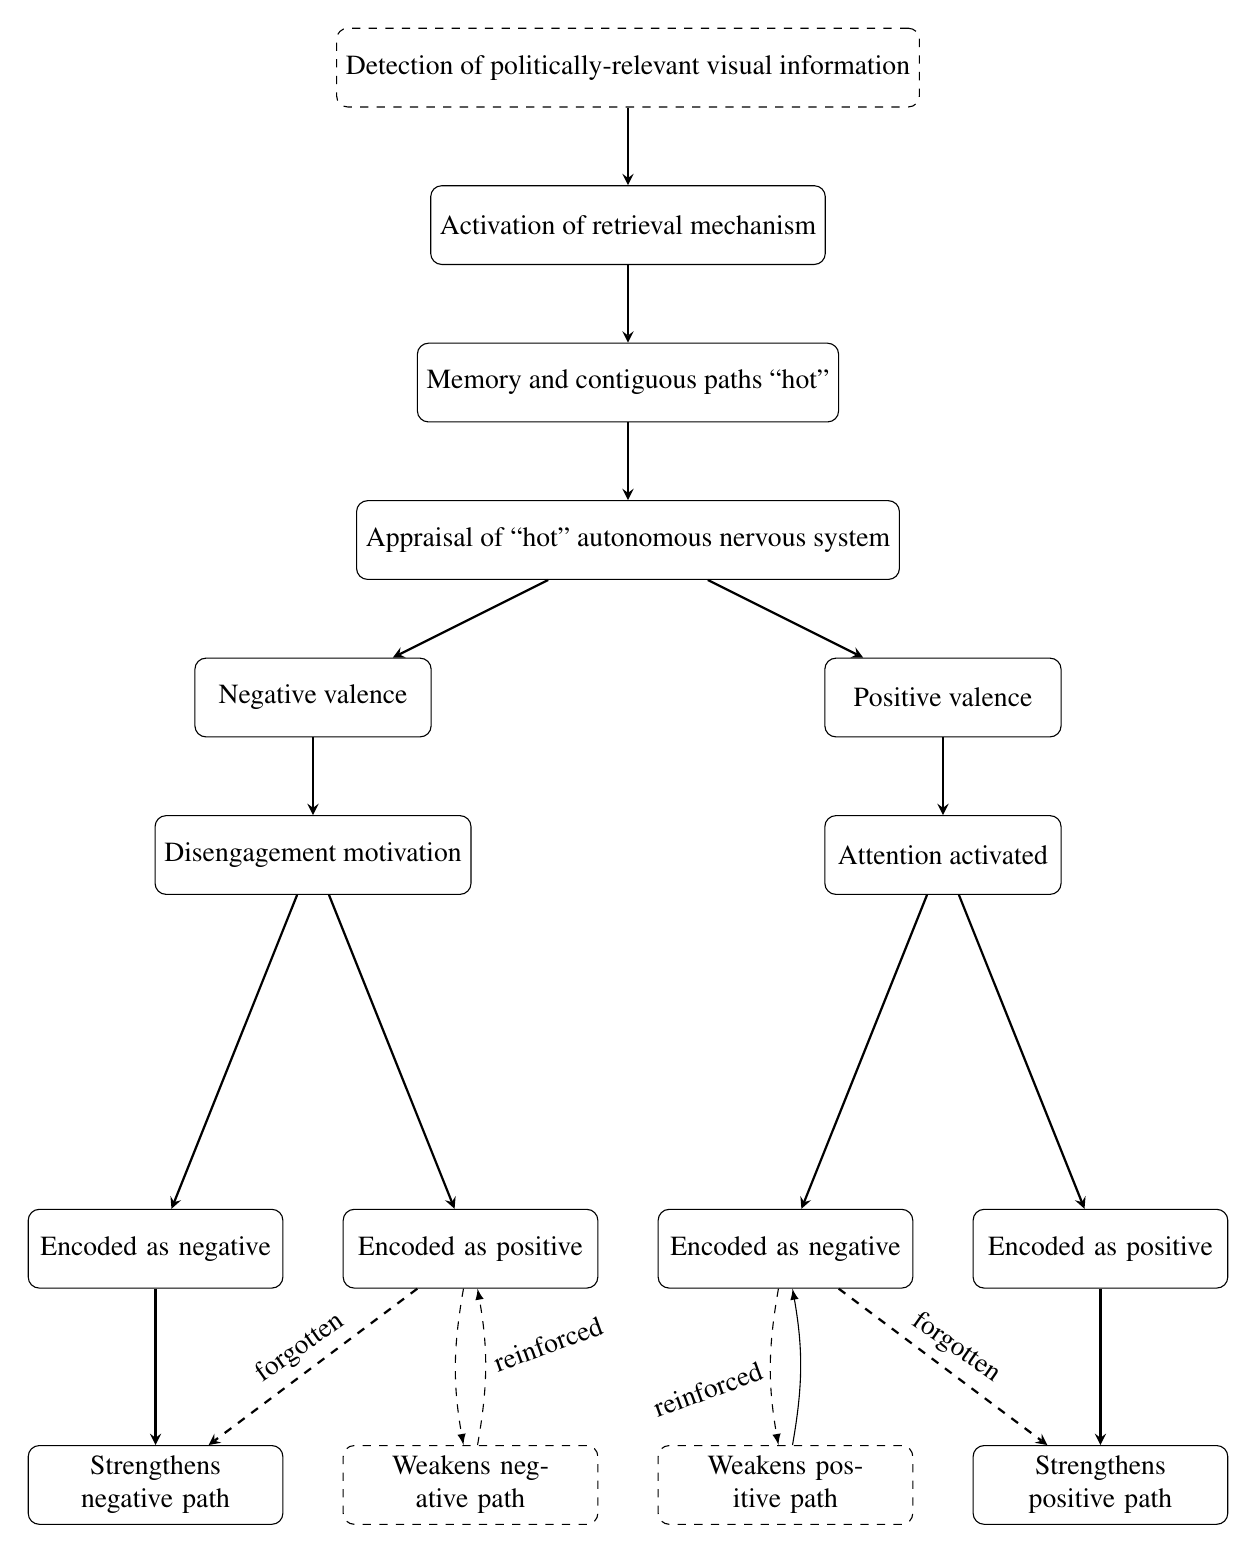
\begin{tikzpicture}[node distance = 2cm]
    \node (start) [startstop, dashed] {Detection of politically-relevant visual information};
    \node (in1) [io, below of=start]{Activation of retrieval mechanism};
    \node (in2) [io, below of=in1]{Memory and contiguous paths ``hot''};
    \node (in3) [io, below of=in2]{Appraisal of ``hot'' autonomous nervous system};
    \node (in4a) [io, right of= in3, xshift = -6cm, yshift = -2cm]{Negative valence};
    \node (in4aa) [io, below of=in4a]{Disengagement motivation};
    \node (in4aaa) [io, below of=in4aa, xshift = -2cm, yshift = -3cm, text width = 3cm]{Encoded as negative};
    \node (in5ns) [io, below of=in4aaa, yshift = -1cm, text width = 3cm]{Strengthens negative path};
    \node (in4aab) [io, below of =in4aa, xshift = 2cm, yshift = -3cm, text width = 3cm]{Encoded as positive};
    \node (in5nw) [io, below of =in4aab, yshift = -1cm, text width = 3cm, dashed]{Weakens negative path};
    \node (in4b) [io, left of=in3, xshift = 6cm, yshift = -2 cm]{Positive valence};
    \node (in4ba) [io, below of =in4b]{Attention activated};
    \node (in4baa) [io, below of=in4ba, xshift = -2cm, yshift = -3cm, text width = 3cm]{Encoded as negative};
    \node (in5pw) [io, below of = in4baa, yshift = -1cm, text width = 3cm, dashed]{Weakens positive path};
    \node (in4bab) [io, below of=in4ba, xshift = 2cm, yshift = -3cm, text width = 3cm]{Encoded as positive};
    \node (in5ps) [io, below of=in4bab, yshift = -1cm, text width = 3cm]{Strengthens positive path};
    \draw [arrow] (start) -- (in1);
    \draw [arrow] (in1) -- (in2);
    \draw [arrow] (in2) -- (in3);
    \draw [arrow] (in3) -- (in4a);
    \draw [arrow] (in4a) -- (in4aa);
    \draw [arrow] (in4aa) -- (in4aaa);
    \draw [arrow] (in4aaa) -- (in5ns);
    \draw [arrow] (in4aa) -- (in4aab);
    \draw [-latex, dashed] (in4aab) to[bend right = 10] node[right, rotate = 20] {} (in5nw);
    \draw [-latex, dashed] (in5nw) to[bend right = 10,] node[right, rotate = 20] {reinforced} (in4aab);
    \draw [arrow] (in3) -- (in4b);
    \draw [arrow] (in4b) -- (in4ba);
    \draw [arrow] (in4ba) -- (in4baa);
    \draw [-latex, dashed] (in4baa) to[bend right = 10] node[left, rotate = 20] {reinforced} (in5pw);
    \draw [-latex] (in5pw) to[bend right = 10] node[below, rotate = 60] {} (in4baa);
    \draw [arrow] (in4ba) -- (in4bab);
    \draw [arrow] (in4bab) -- (in5ps);
    \draw [arrow, dashed] (in4aab) -- node[anchor = south, rotate = 35]{forgotten}(in5ns);
    \draw [arrow, dashed] (in4baa) -- node[anchor = south, rotate = -35]{forgotten}(in5ps);
\end{tikzpicture}
\end{mdframed}
    \caption{Snap-judgement model of politically-relevant visual information}
    \label{fig:snap-judgement_model}
    \floatfoot{Note: Dashed nodes represent the primary innovations of the snap-judgement model.}
\end{figure*}

%What image does this evoke? Do you see just the hat? Do you have memories which suggest that you should associate such visual information with other information? Do you imagine the wearer of the hat being a man, being white, perhaps even wearing cowboy boots? Do you now think you are at an airport in New York City or at an airport in Dallas Texas? Do you know what the message on the hat in white lettering says? Perhaps it says "Make America Great Again". What physical reaction do you have to this image? Perhaps your heart rate increases, perhaps your hands become a bit clammy. Do you feel disgusted, angry, excited? How quickly did you conjure such an image in your mind? How quickly did different parts of that image form? Did the hat and the features of the wearer come faster than the text on the hat and faster than imagining a particular airport? Did you anticpate that the hat was a symbol for a political message?
%
%Visual information is quite powerful. Symbols and visual information conveying a story or ideas have a much deeper root in human evolution than written text. Our brains are optimized to percieve and to associate visual information with memories at remarkable rates. Some estimate that the processing of visual images happen in as little as 13 milliseconds \citep{potter_et-al_2014_app}. Text-based information happens much slower as it follows a linear and ordered process through the brain unlike visual information which can be processed simultaneously in different regions of the brain \citep{vogel_et-al_1986_wp}.
%
%As visual information is efficient, it has an important place in politics. Symbols and colors that represent parties, countries, and ideologies are readily recognizable. The first televised presidential debate is said to be a turning point in the campaign of a young and attractive John F. Kennedy. Yard signs with the name of a political candidate are put up by strong partisans as an expressive act which often succeed at generating valenced reactions from their outpartisan neighbors \citep{makse_et-al_2019_oup}. Even in seemingly non-political ways, observing stereotyped cultural differences between Republicans and Democrats act as accurate visual cues (such as the modal car in the driveway, or whether it is a suburb or densely populated, mixed use neighborhood) of any given neighborhood to make assumptions about the partisan composition of those who live there \citep{hetherington_weiler_2018_hmh}. This work among political psychologists has yet to unpack the particular mechanism by which visual information works in associative memory to take both political and seemingly apolitical information to shift attitudes and behavior. Moreover, as visual information is a much more efficient source than text, it has yet to be studied how it is a more effective means by which people come to accurate and rapid politically-relevant appraisals with only visual information.
%
%This dissertation studies the role of visual information in producing snap judgments about others in reference to their political views. In doing so, I argue that visual information produces faster and stronger affective responses than text-based information. Using an affective memory and hot cognition model, it argues that politically-relevant visual information is encoded as affectively charged in long-term memory. With new political information sparking associative memory, this new visual information is quickly percieved and brought to consciousness along with prior associated memories and their valenced charge. As this information reaches consciousness first, visual information produces a quick, gut-level, and affective snap judgement about the image. 
%
%The implications of such a theory inform not only the way in which political information is processed, but more importantly it identifies the foci. As previous research on political memory and information processing has debated the way in which individuals access and store new political information, the preeminant memory \citep{zaller_1992} and online models \citep{lodge_et-al_1995} of information processing characterize new information as complete and wholistic. Acting within a subsystem, a snap judgement based only on visual information produces an almost immediate barrier if one pre-consciously associates this visual information with negative valence. In taking this view, this model of snap judgements relies on the theory of affective intelligence which suggests that distinctive categories of affect encourage distinctive behaviors.
%
%The model suggests that snap judgements that call particular affectively encoded associative memories influence the degree to which one consciously engages with the new information. Where visual information activates affectively charged associative memories that suggest retreat, the model suggests that attempts to shift foci on other features are less likely. This necessarily means that visual information that activates affectively charged associative memories that suggest approach, will encourage an individual to shift their focus on other features and to engage in conscious processing are more likely. 

%Information is affectively encoded. Early work in psychology demonstrates that visual information often has affective attatchments \citep{cimbalo_et-al_1978_jgp}. These associations with visual information and affect are likely learned. The theory of hot cognition suggests that we rarely learn information through details but rather we can speed up this process through encoding this information \textit{vis-a-vis} affect. As a theory of memory encoding, hot cognition is believed to be important for the processing of political information and the formation of political attitudes \citep[see][]{taber_lodge_2006_cup}. Once stored in long-term memory, this information can be accessed later through similarity which trigger similar neurological patterns.

%We use visual information to make judgements about others. We seek to understand who they are just by the way they dress, the way they carry themselves, and the way they take up space. These features are also expressive. We curate the way we visually present ourselves as a way to represent to our personality. To percieve visual information light passes from the cones and rods in our eyes to our optical nerve, then to our lateral geniculate nucleus in the thalamus to our visual cortex. Once percieved, visual information passes through our brain to spark memories and to reinforce others. Some estimate that the processing of visual images happen in as little as 13 milliseconds \citep{potter_et-al_2014_app}. While it takes longer to connect this information to memory and even consciousness, visual information is powerful and fast. But just how useful are these fast sources of information for understanding politics?
%
%The advent of televised Presidential debates partly contributed to the success of a young and attractive, John F. Kennedy. Some political psychologists connect the role of visual information as a source of political information. \citet{hetherington_weiler_2018_hmh} demonstrate that individuals are able to accurately attribute the partisan leanings of a given neighborhood only with visual information that communicates cultural stereotypes that differ between partisans. \citet{makse_et-al_2019_oup} demonstrate that strong partisans tend to put up yard signs as an expressive act which tend to produce strong valenced reactions among outpartisan neighbors. What remains unclear in such narratives is whether these sources of visual information produce ``snap judgments'' and what the implications of such evaluations have on learning and social interactions.
%
%Politically-relevant information is encoded in long-term memory with the help of emotion. \citet{lodge_et-al_1995} demonstrate that individuals do not store the details of political information in long-term memory, but rather that they encode it as valanced information. This information is accessed through hot cognition, a mechanism whereby this information is stored based upon affectively-charged information. This information is most accessible when similar affectively charged information reminds one of it \citep{taber_lodge_2006_cup}. The process of perceiving politically-relevant information to its presence in consciousness so that it might be encoded is within $1800$ milliseconds \citep{taber_lodge_2006_cup}. Therefore, we should expect that visual information be affectively encoded into long term memory and that this should happen relatively quickly.
%
%Visual information processing is more efficient than text-based information processing. Visual information is processed faster as it is done simultaneously in different regions of the brain as opposed to text-based information which follows a slower, linear, path \citep{vogel_et-al_1986_wp}. This means that visual information is more likely to be an efficient means for generating snap judgements. If we see an individual wearing a ``Make America Great Again'' hat, we are most likely to see the characteristic bright red with white lettering. When we see the characteristic bright red hat with white lettering, we see who is wearing the hat: are they wearing cowboy boots, are they White \footnote{Except for Kanye West}, are they male? Taking this information together, we then have an affective reaction: we are excited to see another Trump voter or we have a reaction of disgust, anger, or even hatred. 
%
%When we have this affective reaction and come to a snap judgement, we have learned about the individual and we have reinforced the views we have of the stereotype of the type of people who were ``MAGA'' hats in public. 
%
%This is a dissertation of snap judgements and their implications.





%Throughout my time in graduate school, I continue to come back to questions involving our understanding of how well (or unwell) the American public is represented in politics. In doing so, I tend to examine how the public gets in the way of their expression of political voice. I started my undergraduate studies with the intention of earning a degree in Biology with the fuzzy goal of studying the human brain or attending medical school to work in neurosurgery. As I took classes on political psychology and political communication, I realized that I could understand how politics affects the brain and how features of the brain influence the way we engage in politics. I knew that I wanted to keep studying those questions for my dissertation.
%
%The literature of affect in politics has a long intellectual history \citep[see][for a discussion]{marcus_2000_arps}. Many early discussions held a normative definition and interpretation of their role. Classic democratic theorists considered the role of the citizen to be that they rationally make decisions and exercise voice based on careful consideration of the facts. These normative interpretations of emotions' role in democratic politics lasted through much of the behavioral revolution in the social sciences, with grand theories of vote choice debating the rationality of the average voter. For the last $4$ or $5$ decades, political scientists leaning more on the literature in psychology shifted their tone. They began to consider emotions as serving functional purposes for memory encoding, retrieval, and its mediatory role in forming political attitudes. As these political psychologists have relied more heavily on the literature in psychology, the definitions and operationalization of effect began to demonstrate the relative lack of consensus about what emotions are and how they work. This mirrors the same challenges experienced by those who study affect in psychology and neuroscience \citep{sander_2013_chhan}. Even with the advent of more objective measures of emotion, definitions of what they are or theories about how they work still are somewhat splintered \citep{sander_2013_chhan}. The two primary ways scholars think of emotions in psychology have their roots in a debate between Charles Darwin, William James, and Walter Cannon. Darwin conceptualized emotions as autonomic reactions to a stimulus from the environment \citep{darwin_et-al_1998}. On the other hand, James and Cannon saw them as the interpretations of autonomic physiological reactions to a stimulus \citep{james_2013, cannon_1927_ajp}. In the study of affect in political science, the two primary theories that reign today are that emotions are either pre-conscious drivers of behaviors or that they are cognitive appraisals of political stimuli. 
%
%Though many political psychologists study affect, there remain many open questions. First among them is how we define emotions. Though there are different interpretations, the literature seems to largely ignore the differences between the way the two major theories of affective politics define politics. Literature reviews on political affect are examples of the subfield's tendency to neglect this.
%
%Relatedly, the literature has seemed to become its own subfield as there seems to be less borrowing from the literature in affective psychology and neuroscience. One implication of this second open question is that our research designs involving questions of affect rarely rely on multiple, simultaneous measures of emotion. Affective neuroscientists tend to rely on the familiar-to-affective-politics-scholars self-reporting of emotions from surveys and survey experiments, as well as neurological processes and physiological reactions. That is, affective neuroscience and psychology detect emotion through multiple measures. Many see emotions as just the neurological processes in both the pre-conscious and conscious brain, but not as the complete picture of the emotional state \citep{ralph_anderson_2018}. The other implication of a less interdisciplinary approach to the study of affect in politics is the loss of interest in clarifying the position one takes in the literature when choosing a particular definition of emotion. Consequently, we risk proposing theories that simultaneously suggest support for both affective intelligence and cognitive appraisal theories of emotion.
%
%Besides questions of concept and measurement, there are many open substantive questions about the role of emotion. Though political psychologists took a more functional approach to study emotion, much of the work has been to understand the role of emotion from the perspective of attitude formation and political knowledge. As the behavioral revolution was underway, scholars of American political behavior characterized the public as unsophisticated partisans \citep{converse_1964}. This characterization continues today \citep[see][as examples]{delli-carpini_keeter_1996,achen_bartels_2016}. In attempts to understand the empirical variation implied by those claims, many have taken emotion as an angle to understand such questions. A smaller group of scholars have studied the role of emotion as motivation for forming behavior and not just attitudes. Interpersonal deliberation is one form of participatory behavior with a rich intellectual history.
%
%Though there is work examining emotions' role in deliberation, the causal process remains somewhat unclear in this literature. In examining what motivates individuals to engage in deliberation in the first place, MacKuen and colleagues \citeyearpar{mackuen_et-al_2010_ajps} argue that anxiety encourages more willingness to engage in conversations with those they may disagree with. Using a different angle, Lyons and Sokhey \citeyearpar{lyons_sokhey_2014_pc} find evidence suggesting that emotion shapes the content of the conversation but cannot find consistent evidence that it motivated the conversation. In retrospectively evaluating a conversation, individuals who tend to report an enthusiastic mood toward politics tend to enjoy deliberating politics more, and those who are angry are more likely to avoid political conversations \citeyearpar{wolak_sokhey_2022_apr}. This work suggests that there is still quite a lot of uncertainty about the causal relationship between emotion and deliberation. Making a similar argument, Neblo \citeyearpar{neblo_2020_apsr} argues that emotion and deliberation are endogeneous. Emotion and deliberation each shape one another. However, as studying their relationship is a relatively small focus for the deliberation and emotion literature, there has yet to be a comprehensive detailing of the way in which emotion and deliberation cause and are caused by one another.
%
%Previous theories that examine informal deliberation wholistically often rely on social psychological theories to motivate their claims. To date, the prevailing comprehensive theory of informal deliberation is rooted in social psychological theories. In a valuable and thorough analysis of the motivations of individuals finding themselves in political discussions, Carlson and Settle \citeyearpar{carlson_settle_2022_cup} argue that instrumental factors and those affecting social relationships explain individual heterogeneity in the willingness to engage in conversation, what they discuss when in the conversation, and the degree to which they engage in social distancing from outpartisans. While prevailing work primarily relied on assumptions about accuracy goals as a primary motivator for deliberation, Carlson and Settle \citeyearpar{carlson_settle_2022_cup} argued that there are also motivations rooted in self-image protection and partisan affiliation. In explaining the effects of deliberation, the comprehensive social psychological theory of informal deliberation suggests that individuals appraise their experience to update their networks and to examine their willingness to make similar choices in whether to engage in a conversation and how to engage in the conversation in the same way under similar circumstances. 
%
%The focus of this dissertation is to propose a comprehensive cognitive theory of informal deliberation. Specifically, this dissertation relies on the Schacter-Singer theory of emotion \citep[see][for a discussion]{sander_2013_chhan}. Where one finds themselves stumbling into a conversation about politics, individuals will experience arousal - which often manifests through a physiological response \citep{carlson_settle_2022_cup, mutz_reeves_2005}. This physiological response is then evaluated consciously and assigned a label that reflects the valence of the emotion. This valence suggests to the individual which course of action is most appropriate to reduce the degree of arousal. This process continues throughout the experience in the conversation. At the close of the conversation, the theory of hot cognition would suggest that the valence and arousal one experiences at that time will lend itself to the memory of the event and will inform future reactions to similar stimuli \citep[see][]{taber_lodge_2006}.
%
%Specifically, I examine the motivation to engage in a political conversation with the view that it arises from an affective response to a stimulus. Those who have strong physiological reactions to realizing a conversation they just walked into will take note of what that physiological reaction implies. What that physiological reaction implies falls on two dimensions: the magnitude of the difference between their current state and baseline state (arousal) and the directionality of that response (valence), whether it be inductive of anxiety, fear, anger, or enthusiasm, or joy. Once the level of arousal is determined, and the individual assigns a label for the emotion one is feeling, the individual has the choice of whether to find an excuse to leave quickly or to let it play out. As they hear more from others in the conversation and understand the topic of discussion, the online model of information processing would suggest that individuals would access information or encoded memory through recollection of the emotional state associated with that information \citep{taber_lodge_2006}. That then determines whether and how someone might jump in to express their point of view. As the conversation comes to a close, one takes stock of the experience that just occurred by assessing their emotional state throughout the process. Then that information informs one on how to encode whether that conversation was positive or negative, whether it is encouraging for whether or not to engage in future conversations with similar dynamics and on similar topics, or whether to take on some other form of politically relevant behavior such as a reluctance to talk to specific people in the future or about a particular topic, or even politics altogether.
%
%The contribution, as I see it, is not just substantive but also hopefully clarifies the position that those studying affect in politics have taken from the perspective of those in other disciplines. As I will outline in the dissertation's first half, it should put perspective on the more significant debates that need to occur as we continue to examine emotion. While borrowing a different theory of emotion is not as popular among political scientists, it seeks to act as an alternative (at best) or at least play a devil's advocate role to stretch the validity of the two standard models used by political psychologists (at worst). With this goal, it meets another. The theory implies physiological, neurological, and cognitive measures of emotion as they operate in a distinct and ordered fashion.
%
%IGNORE THE OUTLINE SECTION FOR NOW. MAKE SURE TO HAVE ARGUMENT NAILED DOWN. ONCE COMFORTABLE WITH THE DIRECTION, THEN THERE WILL BE MORE STRATEGIZING ON THE SPECIFICS OF TOPICS FOR THE CHAPTERS AND RESEARCH DESIGN.
%
\section*{Outline of empirical chapters}
    \subsection*{Chapter 1}
        \subsubsection*{Argument}
Can something as simple as color influence a campaign or even one's political attitudes? Political scientists have largely ignored such simple visual information despite their focus on party branding and communication strategies. One potential reason for this being is that the literature still largely disagrees over whether campaigns, on the whole, matter for shaping electoral outcomes and the attitudes of voters \citep{broockman_kalla_2022_ajps}. I argue, however, that though color may not determine electoral outcomes, it may still be an important piece of visual information that encourages learning by voters. I also test whether it influences how people respond to political surveys as they are often used for polls which are a cottage industry partially as a result of the popularity of election forecasting.

Since the 2000 election cycle, it has become commonplace for political candidates to rely on the colors red and blue as part of their campaign branding strategy. The use of the colors red and blue to distinguish between Republicans and Democrats on electoral maps became more common place starting in the 1970's \citep{elving_2014_npr}. Outside of this, the literature connecting simple visual information and color is relatively sparse. I attribute this to most studies used in political psychology as focusing on the generalizability of their treatments and for the theories to focus on visual and complex visual information.

The snap-judgement model offers predictions about how individuals should process simple visual information such as colors. Colors are first perceived as a particular set of wavelengths which trigger particular sensory receptors in the back of one's eye. This is converted into an electrochemical message that goes to the thalamus and into the primary visual cortex in the back of the brain. To make sense of this information, our brain accesses memories containing similar information which are affectively encoded \citep{cimbalo_et-al_1978_jgp}. Beyond the connection between particular colors and affect, the use of colors to distinguish political parties are so common-place that individuals likely access affectively encoded referential memories as well.

In non-political settings, we may unconsciously associate colors, \citep[see][]{mehta_zhu_2009_s}, such as blue with ``happy'' and pleasure and red as ``sad'' \citep{d'andrade_egan_1974_ae}, arousing \citep{valdez_mehrabian_1994, mehta_zhu_2009_s, elliot_maier_2012_aesp}, and angry \citep{epps_kaya_2004, elliot_maier_2012_aesp}. Indeed, in a political context, such visual information activates pre-conscious processes that may diverge from that. These colors hold important meaning beyond the raw affect they engender. Republicans report that they prefer the ``Republican red'' more than they do the ``Democrat blue'' \citep{schloss_palmer_2014_pbr}. That is, the colors red and blue in a political context are likely to make the neural pathways related to one's partisanship ``hot''. Some evidence suggests that there is indeed a strong link between ideology and color \citep{casiraghi_et-al_2022_pp}, and that these associations are stronger in Western European countries and for parties that are relatively well-established. As simple visual information such as color is processed at remarkable speeds, it likely occurs even faster as primes of group identity speed up pre-conscious processing of information \citep{lodge_taber_2013_cup}. 

Once these politically-laden neurological pathways are activated, the affect associated with these nodes along the path will be appraised by the body and will encourage a particular physiological reaction which are themselves associated with particular behavioral outcomes. Where these colors activate associations with the out-group, an individual is likely to have a physiological response encouraging the disengagement motivation. Where the color activate associations with the in-group, an individual will experience a physiological response encouraging an approach motivation. 

As this is pre-conscious processing, it will put an individual in a ``mental framework'' or in a cognitive state that encourages biased information processing, both pre-consciously and consciously \citep{lodge_taber_2013_cup}. However, this is continually updated with more information. Where new information comes in such as context, or a conversation, or just new simple visual information, the mental state that the snap-judgement put one in, will update with this information; it will either strengthen the path initiated by the snap-judgement, or it will attenuate the strength of the path. As this experience is forgotten, the effects of strengthening or attenuating the strength of the path will dissipate. If it is reinforced, then the effects will hold and may even strengthen.

In line with the snap-judgement model, some evidence suggests that the use of red and blue in political messages activate partisan biases in Spanish samples \citep{maestre_medero_2022_pr}. As the colors red and blue hold important meaning in political contexts, these colors pre-consciously activate pathways that associate those colors with particular partisan or ideological groups. These associations are stronger the more established the party is \citep{casiraghi_et-al_2022_pp}. That is to say that these associative networks are stronger and easier to access in pre-conscious processing. 

Applying the snap-judgement model to such a case yields a handful of expectations:
\begin{itemize}
    \item[$H_1$:] Individuals associate the color red with Republicans and the color blue with Democrats.
    \item[$H_2$:] When exposed to stimuli containing a political message and colors with political meaning, individuals will process the color before the message.
    \item[$H_3$:] When engaging with the colors red and blue, they will have valanced reactions to such stimuli as the result of the identity-based meaning associated with the stimuli.
    \item[$H_4$:] When a political message paired color is combined with contextual information, the color will meaningfully shape the evaluations of the stimuli.
    \item[$H_5$:] The mediating effects of the contextual information will persist so long as the memory of the stimuli are reinforced, but will shortly dissipate without such reinforcement.
    \item[$H_6$:] Surveys that offer a UX that offers simple contextual information about the organization conducting the survey will experience higher rates of survey non-response and insincere responses among those who hold negative \textit{a priori} views of the organization.
\end{itemize}

        \subsubsection*{Research Design}
Before examining whether this complex process implied by the snap-judgement model occurs, it is important to first establish whether individuals associate particular colors with groups. Studies that associate color with parties are largely focused on european samples \citep[see][]{casiraghi_et-al_2022_pp,maestre_medero_2022_pr}. It is unclear, however, how engrained these associations are among Americans. 

To examine $H_1$, I propose conducting an online survey where I ask respondents to match visual information they associate with different political groups. These visual groups include the parties: Republicans and Democrats, but also prominent groups such as the Sierra Club, the Proud Boys, anarchists. This visual information is a combination of logos such as an elephant - associated with the Republican party, a donkey - associated with the Democratic party, trees - associated with the sierra club, the rooster symbol - associated with the proud boys, the characteristic A associated with anarchists. These images will be monochrome to isolate the effects of the image. The visual information to be matched with these various groups will also be color: Red and white - associated with Republicans, Blue and white - associated with Democrats, green and white - associated with the sierra club, black and yellow - associated with the proud boys, and red and black - associated with anarchists.

To study $H_3$, I need to examine whether people experience affectively valanced reactions to colors in both political and apolitical settings. It is important to examine whether these responses are different depending on context as it establishes whether consuming such visual information in different contexts activate different neurological paths. To do this, I will randomly assign experimental participants into different conditions. 

In the political context condition, participants will start the experiment by responding to a political attitudes questionnaire; a battery that asks them a number of questions prompting them to express their political views on policy issues. In the apolitical conditions, participants will skip the political attitudes questionnaire and will experience the treatment. 

The treatment will be a square box with the color red, blue, or grey. The treatment will ask participants to also report whether it is a positive or negative color. It will record how long it took for participants to report the valence. Like the implicit attitudes test, the goal of this is to examine quick and immediate valanced reactions to the treatment. There will be a number of burn-in rounds where participants will see other colors such as orange, grey, and yellow as a way to get a baseline - this is important given the individual-level heterogeneity in speed that may come about from unobserved factors such as the use of a laptop, monitor specifications, the use of a mouse and trackpad or arrows on the keyboard, etcetera. 

After the burn-in rounds and a few rounds with the treatment, participants are asked to provide responses to about five open-ended questions asking about what they had for their most recent meal, what their last vacation was, what was the last thing they bought, what day of the week elections tend to be held on in the United States, and what was the last bit of news they had heard about American politics. The point of these questions is for detecting insincere responses. As experiments suffer mightily from attentive subjects, from those who are indeed American citizens, and from trained bots, evidence suggests that - beyond the use of attention checks, identifying duplicate IP addresses, and identifying ``speeders'' and ``turtles'' - the use of open-ended responses are an effective way at identifying subjects providing insincere data points \citep{kennedy_et-al_2021_poq}. 

To establish another critical assumption of the model is whether people do pick up on this simple visual information faster than messages, $H_2$. Though the psychology literature suggests that may be the case, this is still an untested assumption in political settings. As political messages communicate identity-based information, messages may go through the pre-conscious process faster than simple visual information.

To test whether this assumption holds up, I first ask participants a series of questions in a political attitudes questionnaire. In the questionnaire, participants are asked about their partisan identification. This should prompt them to think of their in-group, what partisan group they belong to. As primes related to one's in-group yield faster responses to messages shared by the in-group, I use this information to conduct a blocked three-arm experimental design.

Participants will be randomly assigned into one of three conditions. In each of these three conditions, they will see a box with a color background and in the foreground a message to vote for either Joe Biden or Donald Trump. For those who reported that they were Republicans, they will receive a message to ``Vote for Trump''. If the subject self-identifies as a Democrat, they will receive a message to ``Vote for Biden''. The conditions vary in which color is in the background of this message. The three conditions are that the background uses either the color red, blue, or grey. Like I did in the other study, participants will be asked on the same screen to report the valence of the image and the length of time it takes for the subject to respond will be recorded. They will only do one round with the treatment to reduce introducing bias captured by participants realizing it is the same message but with a different color background. Before the treatment, they will receive the same burn-in practice to establish a baseline for the participants speed. After the treatment, participants will be prompted to respond to the same five open-ended questions as participants in the other study. 

I will then perform another study to examine whether contextual information mediates the effects I expect to find in the previous studies. To examine $H_4$ and $H_5$, I propose a study that includes more complex contextual information. In the context of this study, the more complex information would be to place the treatments used to establish $H_2$, in a public space and in front of a house in a neighborhood. The dependent variables of interest here are not necessarily the valence it generates, but the valanced pre-conscious evaluation of the candidate owning the yard sign and the presumed owner of the home displaying the yard sign (in the neighborhood conditions only). Leveraging the conditions used to examine $H_2$, this not only allows for me to evaluate the mediating effect of the more complex visual information, but it also allows for me to examine the pre-conscious effects of color relative to those of the message on the yard sign.

The way that I intend to construct the visual information is by using validated images of neighborhoods and public spaces that the public view as partisan. As \citet{gebru_et-al_2017_pnas} demonstrate through the use of google images, features of neighborhoods such as the prevalence of pickup trucks relative to sedans betray the partisanship of the neighborhood. By collecting images from google streetview, I can collect images of neighborhoods that break solidly Republican or Democratic. I then will validate these choices with a small sample of human coders who will guess how partisan the neighborhoods in the images are. From those neighborhoods that have the most intercoder reliability representing a widespread belief of clear partisan leanings, I will then photoshop the image of a yard sign varying the message and color treatments.

To examine the duration of these effects, some participants will be recontacted each day for two weeks. Half of the participants, randomly chosen, will be recontacted once at the end of the two week period and the other half of participants will be recontacted each day. During recontact they will be asked to choose features that they remember from the initial treatment they received. As they will after the treatment, they will be asked a series of questions about the valanced reactions the subjects had toward the candidate owning the yard sign and the owner of the house displaying the yard sign. This will allow me to examine the duration of these mediating contextual effects and to examine whether this duration of the effects are dependent on frequent recall of the original stimulus.

I then will conduct a final study to examine whether the model has something to say about survey non-response and insincerity rooted in respondent partisanship. I AM NOT SURE HOW TO DO THIS EXACTLY... LIKE HOW WOULD I GET AT NON-RESPONSE WITHOUT INFORMED CONSENT?

        \subsubsection*{Proof of concept: A pre-test}

I conducted a pre-test in November 2019 with a sample of over 400 undergraduate students at a medium-sized University in the northwestern region of the United States. Students were recruited if they were enrolled in a political science course and were offered extra credit for their participation in the study. The study asked participants to participate in $5$ survey experiments administered by those affiliated with the university's college-level unit. These other survey experiments were focused on capturing local policy issues around urban design, criminal justice, and probing participants about political participation in local and national-level elections. Participants were asked to participate in my survey experiment after one that examined their levels of political participation in local, state, and national elections.

\Cref{tab:descriptive_stats} presents the descriptive characteristics of the sample. The sample is primarily White with over $80\%$ self-reporting that they are White(coded as: 0 = non-White, 1 = White). The sample also skews slightly female on sex with about $60\%$ of the sample reporting that they are female (coded as: 0 = Male, 1 = Female). The sample also, unsurprisingly, skews young with the average respondent reporting an age of about 22 years old. The average respondent also appears to be an independent but leans Republican (coded as: -3 = strong Democrat, -2 = Democrat, -1 = leans Democrat, 0 = Independent, 1 = leans Republican, 2 = Republican, 3 = strong Republican).

I randomly assign participants into three conditions. The conditions prompt subjects to ``Imagine that [they] are driving along a road and see this yard sign'' with the same message ``Vote for Riley''. The conditions vary on the color of the background for the image\footnote{The images used for the treatments and the particular wording for the dependent variables are included in the Appendix}. In the control condition, the background was white. Then I had a red yard sign and blue yard sign condition. On a separate screen participants were asked a series of questions acting as outcomes of interest.

To provide a preliminary test of $H_1$, I ask participants to report whether the candidate was a ``Republican, Democrat, or Independent''. Though it does not capture pre-conscious processes, I also wanted to capture the valence of the presumed out-or-co-partisan yard sign engenders for subjects. To do this, I ask respondents whether they would ``seek out more information about the candidate'', ``avoid the candidate'', ``or vote for the candidate''. Subjects could respond to one of the three questions with a ``yes" or ``no'' response. I then combine these questions into a single measure of the subjects' valanced response directed toward the candidate. Those that reported that they would vote for the candidate or seek out more information, were coded as 1. Those who reported that they would avoid the candidate were coded as -1. And those who reported some combination that represents mixed views or some degree of ambivalence were coded as 0. 

I also wanted to examine whether these valenced reactions to the yard sign were also directed toward the presumed neighbor who displays the yard sign. I asked participants to respond ``yes'' or ``no'' to whether when ``imagining this yard sign on a neighbor's lawn" whether the subject would want to ``talk to the neighbor to seek out more information about the candidate'', ``tell the neighbor that you want to vote for the candidate'', or to ``avoid the neighbor''. As I did with my outcome of valenced response directed toward the candidate, I also combined these three questions. Those who reported that they would want to avoid the neighbor were coded as a 0 and those that indicated that they would want to interact with the neighbor were coded as a 1. 

I test whether participants presumed that the candidate was of a particular partisan persuasion just based on the color choice of the yard sign alone and whether this moderated by the partisanship of the participant influenced reported valenced reactions directed the owner of the sign and a neighbor displaying the sign. I create two dummy variables of the treatment the subjects recieved: whether or not they had the blue or the red yard sign treatment. The control condition is treated as the baseline condition when including both dummy variables in my model. 

To examine whether subjects presumed that the fictional candidate is affiliated with a particular political party, I fit a model using a cumulative link function from the logistic distribution and specify a prior location of the $R^2$ - which represents the proportion of variance the model explains for the discretized latent variable - with an average $R^2$ of $0.3$ when the predictors are at their sample means \citep[see][Chapter 15]{gelman_et-al_2021}. I assume this about the $R^2$ as I recognize that color is not going to explain all of the variation in the subjects' ability to detect partisanship, however, my theory suggests that it should have some meaningful impact. Therefore, I choose an expected value of $0.3$, representing that I expect that my treatments should predict about $30\%$ of the variation. I also assume that my errors are normally distributed with a mean of zero. The model is fitted using $6$ chains and $2000$ iterations. The results are presented in \Cref{tab:pre-test_models}.

\input{../figures/chapter_1/pre-test/chapter_1_pre-test_models.tex}


The results suggest that there is some \textit{preliminary} support for my expectation that individuals associate red and blue with Republicans and Democrats. The first column of \Cref{tab:pre-test_models} suggests that individuals in the treatment with the Red yard sign were more likely to guess that the candidate was a Republican, despite having \textbf{no} information about the candidate other than their name and the color of their yard sign. Those in the blue yard sign treatment were more likely to assume that the candidate was a Democrat. The credible intervals for these estimates can be interpreted as the probability that the true estimate is contained in the interval. As neither of these overlap with zero, it is quite plausible that these estimates are not zero.

With confidence that the subjects associate the yard signs with the candidate's partisan affiliation, I turn my focus to their evaluations of the owner of the yard sign and the neighbor who display the yard sign. I make the same assumptions with the model of candidate evaluations given the treatment. As the outcome of interest is a ordinal categorical variable, I specify a cumulative link function from the logistic distribution and specify a prior location of the $R^2$ with an average of $0.3$ when the predictors are at their sample means. As I coded my outcome for the neighbor evaluation as binary, I specify a cumulative link function from the logistic distribution and rely on the default uniform distribution as my prior - which represents that I expect a coefficient on any real number line is equally likely as another. The results of these two models are included in the second and third columns of \Cref{tab:pre-test_models}.

Column 2 presents results suggesting that among Republicans recieving the red treatment, they are more likely to indicate that they have a positive valence toward the candidate. We see that while Democrats recieiving the blue treatment are more likely to also report a positive valence toward the candidate, the effect is plausibly zero. This may be an artifact of asymmetric political polarization. Some scholars suggest that Republicans are much more group-oriented than Democrats \citep[see][]{lupton_et-al_2020}, these results may fit with such a narrative. Republicans are reactive to those they may presume to be a co-partisan in a way that Democrats do not appear to be as reactive in a similar magnitude.

Column 3 presents results that we might have expected. That is, Republicans recieving the red treatment were more likely to report that they would want to interact with a neighbor who are displaying the red yard sign and that Democrats would want to interact with a neighbor who are displaying the blue yard sign. Neither of these effects appear to be plausibly different than zero, however. These results could possibly be explained by characteristics of the respondent and the outcomes measured. Those who are more extraverted may be more willing to interact with a neighbor about a yard sign that they posted, which will affect whether they are willing to ask a neighbor more about the candidate or to tell the neighbor about their support for the candidate. For those who are less extroverted, these ``approach" behaviors may be unpalatable not because of the treatment. In other words, I have a confound that I did not collect data on. It also appears that there was a steep drop-off in the number of participants who responded to these questions with an $N$ of only $267$ relative to the other two models which have an $N$ over $400$. 

The evidence from this pre-test is limited. The experimental design is not testing pre-conscious evaluations. The treatments are explicitly political and was conducted on a convenience sample of those enrolled in political science classes. The ability for individuals to associate partisanship with the treatments are likely overstated. The sample is also quite unrepresentative, so inference is certainly threatened. As I discussed with the third model, I also have omitted variable bias as the result of my outcome being a better measure of approach behaviors for those who are extroverted. 

Though there are problems with the design here, it does serve some purpose for this prospectus. It demonstrates, that dispite its problems, that at some level, when thinking of poltics, color can betray information. It also provides a useful first test of a possible research design to examine what this particular design can and cannot tell me about my proposed mechanism. 

    \subsection*{Chapter 2}
        \begin{itemize}
            \item[2.1] Lay out expectations 
            \begin{itemize}
                \item Visual information tends to be a lot more complicated than just seeing a yard sign in isolation.
                \item We often can use visual information about the space we are in to help us access memories.
                \item The spaces we are in have lots of political meaning to them and this can be detected visually.
            \end{itemize}
            \item[2.2] Can people pick up on the politics just by looking at a space that they are in?
            \item[2.3] What do people focus on when they see these things?
            \item[2.4] Do the things that people notice that have political meaning generate strong reactions?
            \item[2.5] Based on what they notice and what their reaction is to it, does it influence whether they become more attentive, want to retract?
            \item[2.6] If we provide information about the people that are in that space and are involved in shaping that space, can we mediate people's initial reactions? How long do those initial evaluations last? Can we reinforce it to make these mediating effects last longer?
        \end{itemize}
    \subsection*{Chapter 3}
        \begin{itemize}
            \item[3.1] Lay out expectations
            \begin{itemize}
                \item The model also has applicability for influencing whether someone engages in a informal political conversation, how the conversation plays out, and what the lasting impacts of the conversation is.
            \end{itemize}
            \item[3.2] If we have people have conversations with those that have politically-related attire, what are people's reaction to it, if we let people do what they want, do they engage in the conversation; what do they talk about if they do talk? If we force a conversation to happen, what do they talk about? What is their affective reaction to the prospect of having this conversation in both conditions? Do they express more polarized views afterwards?
            \item[3.3] What if we make these visual cues of what the conversation partner is wearing smaller? Do people still pick up on partisan cues like key chains or laptop stickers? What are the effects on motivation to engage in conversation, on the topic of the conversation, and the effects of the conversation afterwards? Are these effects long or short term? If we reinforce them by reminding people of this interaction, do the effects persist? Can they reduce people's valanced attitudes toward those like the person they interacted with?
        \end{itemize}
%How can we measure emotion and how can we do it during a political conversation? Thus far, self-reported measures of one's emotional state requires some degree of cognitive processing. That is, when one is asked how they are feeling or what emotions they are experiencing in response to a stimuli, this necessitates some degree of cognitive processing to evaluate one's emotional state. While I have few doubts these measures are relatively accurate, this measurement strategy limits our ability to detect emotion as deliberation is occurring.
%
%As emotions are measured after a deliberation has occurred, we are likely missing a significant amount of information. Pre-treatment (or pre-conversation) measures of emotion probably do a good job at identifying the emotions present to motivate the conversation. However, with pre-and-post treatment measures of emotion, we are hard-pressed to make claims that these emotions are the ones felt through different stages of the conversation. These emotions are likely to be either emotional states at their end point. But we do not currently know whether these assumptions are indeed true and whether they have consequences for the claims we are making!
%
%Furthermore, these measures on their own also are a very specific conceptualization of emotion. As the discussion in the introductory section highlights, the emotions we are identifying are likely to be better conceptualized as ``feelings''; which are only part-in-parcel of the emotional state. 
%
%Using a combination of neurological, cognitive, and physiological measures of emotion, we not only will increase our capacity to detect variation in emotion over time, but we will also have a better picture of the emotional state as a whole. 
%
%This first chapter is likely to do the most in terms of pushing the argument of measurement
%        \subsubsection*{Research Design}
%
%Won't get into this too much just yet until I have the argument nailed down a bit more.
%
%    \subsection*{Chapter 2}
%The motivation for this chapter will be based on following emotions throughout political conversation using the validated measure from chapter 1. It will examine how emotions motivate participation in a political conversation, how emotions are shaping the conversation's content, and how they shape retrospective evaluations of the conversations' purpose and value to the subjects.
%        \subsubsection*{Argument}
%        \subsubsection*{Research Design}
%    \subsection*{Chapter 3}
%The motivation for this chapter will examine the way that agreement and expertise contributes (or doesn't) to imitation. This imitation can be interpreted as the perceived emotion of a discussion partner and someone's desire to detect it, identify it, and to try to imitate it as part of a desire for belonging in the social group or to reduce conflict. The chapter will then discuss the conditions under which this does or does not work.
%        \subsubsection*{Argument}
%        \subsubsection*{Research Design}
\newpage
\bibliographystyle{apsr}
\bibliography{C:/Users/damon/Dropbox/bibliographies/representation/deliberation.bib,C:/Users/damon/Dropbox/bibliographies/information_processing/interest.bib,C:/Users/damon/Dropbox/bibliographies/information_processing/emotions.bib,C:/Users/damon/Dropbox/bibliographies/representation/attitudes.bib,C:/Users/damon/Dropbox/bibliographies/representation/knowledge.bib,C:/Users/damon/Dropbox/bibliographies/neuroscience_biopolitics/neuroscience/affective_neuroscience.bib,C:/Users/damon/Dropbox/bibliographies/representation/vote_choice.bib,C:/Users/damon/Dropbox/bibliographies/information_processing/motivated_reasoning.bib,C:/Users/damon/Dropbox/bibliographies/representation/trust.bib,C:/Users/damon/Dropbox/bibliographies/neuroscience_biopolitics/neuroscience/visual_information_processing.bib,C:/Users/damon/Dropbox/bibliographies/representation/polarization.bib,C:/Users/damon/Dropbox/bibliographies/representation/participation.bib,C:/Users/damon/Dropbox/bibliographies/representation/elite_cue_taking.bib,C:/Users/damon/Dropbox/bibliographies/neuroscience_biopolitics/neuroscience/memory.bib,C:/Users/damon/Dropbox/bibliographies/stereotypes/party_stereotypes.bib,C:/Users/damon/Dropbox/bibliographies/representation/partisanship.bib,C:/Users/damon/Dropbox/bibliographies/representation/ideology.bib, C:/Users/damon/Dropbox/bibliographies/methods/survey_design.bib,C:/Users/damon/Dropbox/bibliographies/methods/glm_mle.bib}

\newpage
\section*{Appendix}
        \subsection*{Chapter 1}
            \subsubsection*{Pre-test}
\begin{figure}[H]
    \includegraphics[width = 50mm]{../data/chapter_1/pre-test/blue_treatment.jpg}
    \includegraphics[width = 50mm]{../data/chapter_1/pre-test/red_treatment.jpg}
    \includegraphics[width = 50mm]{../data/chapter_1/pre-test/white_treatment.jpg}
    \caption{Treatments}
    \label{fig:treatments}
\end{figure}


\input{../figures/chapter_1/pre-test/chapter_1_pre-test_descriptive_statistics.tex}

\end{document}